\documentclass[conference]{IEEEtran}
\usepackage{cite}
\usepackage{amsmath,amssymb}
\usepackage{graphicx}
\usepackage{booktabs,tabularx,array}
\usepackage{xcolor}
\usepackage[hidelinks]{hyperref}
\urlstyle{same}
\newcolumntype{Y}{>{\raggedright\arraybackslash}X}

\newcommand{\todo}[1]{\textcolor{red}{\textbf{[#1]}}}

\begin{document}

\title{Class-Adaptive Data Augmentation for Road Damage Detection}
\maketitle

% \begin{abstract}

% \end{abstract}

\begin{IEEEkeywords}
road damage detection, data augmentation, class-adaptive learning, augmentation policy, object detection
\end{IEEEkeywords}

\section{Introduction}

Accurate detection of pavement defects are important components of roadway condition assessment, providing information needed to evaluate pavement deterioration and guide maintenance decisions. Traditionally, these assessments have relied heavily on manual inspections, which can be labor-intensive and difficult to implement consistently across extensive road networks. Advances in deep learning have created opportunities to automate this process, with promising results in pavement damage detection and classification~\cite{shang2024automated,zheng2024deep,vision2025inspection}. Despite this progress, achieving reliable performance under varying roadway and image acquisition conditions remains challenging. Differences in illumination, pavement texture, camera perspective, and defect appearance introduce considerable visual variability that may not be adequately represented during model training. This challenge is further complicated by the visual similarities among pavement damage categories, where distinctions often depend on specific geometric and structural characteristics, such as crack orientation, connectivity, and spatial distribution. Consequently, improving model generalization requires accounting for variations in pavement appearance while preserving the visual features that distinguish individual damage categories throughout the image.

Data augmentation offers a practical means of addressing this challenge by introducing controlled variations into training images, allowing models to learn from a broader range of visual conditions without requiring additional data collection. However, the effectiveness of this approach depends not only on the diversity of the transformations applied but also on their ability to preserve the characteristics that define each damage category. For example, geometric transformations may alter the directional features separating longitudinal and transverse cracks, while excessive blurring or occlusion can obscure the fine structural details of interconnected cracks. These effects suggest that the same transformation may provide useful variability for one damage category while compromising essential visual information in another. In detection, this tension arises within a single training image rather than only between images: standard pipelines typically transform the whole frame, so every damage it contains receives the same transformation. As such, a transformation that helps the detector recognize one damage category may degrade another category in the same image, and augmentation policies applied uniformly across all classes may introduce variations that are beneficial to some categories but detrimental to others. Such differences may also be overlooked when augmentation effectiveness is assessed primarily through aggregate performance, as improvements in aggregate accuracy can coexist with reduced performance for individual classes~\cite{kirichenko2023}. This motivates the need for augmentation strategies that account for class-specific sensitivities to different image transformations and can act on each class within a multi-class image.

Existing augmentation methods have progressively addressed this limitation. AutoAugment and RandAugment optimize or control augmentation policies primarily through shared transformation strategies~\cite{cubuk2019auto,cubuk2020rand}, and detection-specific extensions add operations that act on annotated boxes or adapt to object scale~\cite{zoph2020det,chen2021scale}, but their policies are not conditioned on object category. Class-aware approaches recognize that different categories may require distinct augmentation policies~\cite{tsuchiya2019,yoo2023,cheung2022adaaug}, and road-damage detection work has varied augmentation by damage type through probabilities set before training~\cite{rdd_detectron2}. Nevertheless, policies determined before training cannot directly respond to changes in model sensitivity as learning progresses. Online approaches, including CTAugment and CUDA, address this issue by adapting augmentation using feedback from the evolving model~\cite{berthelot2020,ahn2023cuda}. However, CTAugment pools feedback across classes, while CUDA maintains a class-level severity state; both are formulated for classification, where each training sample carries one label, so neither specifies which class's state should govern an image that contains several. This distinction matters because a detector may tolerate strong blurring for one damage class while another, thinner class loses the structure that identifies it. A single state applied to the whole image forces a compromise between them, potentially imposing unnecessary restrictions on beneficial transformations for one class or excessive distortion on the other.

These limitations motivate an augmentation framework that accounts for damage category, the detector's evolving response, and the region being transformed. The proposed framework groups connected overlapping boxes and applies one consistent edit to each selected group. Paired reference and transformed images provide class-specific feedback for photometric and blur/noise operations. Detection retention constrains strength for every class represented in the group, while transformation-induced loss guides family selection. Separate groups can therefore follow different policies, while classes sharing pixels retain a joint constraint.

The central hypothesis is that online class-conditioned control, applied to local groups of damage boxes, improves overall and per-class detection relative to shared augmentation policies. This hypothesis requires evaluation on unaugmented images, including scenes with multiple and overlapping damage classes. To investigate it, we propose the following framework, mechanism, and evaluation protocol:

\begin{enumerate}
    \item An online class-adaptive augmentation framework that regulates transformation strength and family selection by damage category and applies them locally in multi-class road-damage images, with joint tolerance constraints for overlapping boxes.
    \item A feedback-driven adaptation mechanism combining per-class detection retention for strength regulation with transformation-induced loss for family selection.
    \item A controlled evaluation protocol on RDD2022 to characterize damage co-occurrence and class-dependent augmentation sensitivity, separate the effects of local application and class conditioning, and assess detection performance and computational overhead.
\end{enumerate}

\section{Related Work}
\label{sec:related}

The use of data augmentation in pavement damage recognition has developed around the need to obtain informative training examples from limited annotated images. Road-specific studies have approached this need through both the choice of transformations and the construction of additional samples. Tsuchiya \emph{et al.}~\cite{tsuchiya2019} compared augmentation methods by their influence on class-level results and used the selected methods to expand the training data. Aghayan-Mashhady and Amirkhani~\cite{aghayan2024} investigated bounding-box augmentation and generative adversarial synthesis, examining the effect of unrealistic examples on road-damage detection. Detection systems built on multi-country road-damage data tie augmentation more directly to damage types and instances: one Detectron2 and Faster R-CNN system set augmentation probabilities for each damage type and country from data exploration and tested GAN-generated damage patches~\cite{rdd_detectron2}, while a content- and perspective-aware cut-and-paste method accounts for road location and perspective when placing damage instances~\cite{rdd_cutpaste}. Their findings motivate examining augmentation through both the variation it introduces and the damage information retained in the transformed image. The design of the augmentation policy therefore matters alongside the number of examples it produces.

Choosing suitable transformations becomes more difficult as the number of operations, application probabilities, and magnitudes increases. Automatic augmentation methods address this problem at different levels of complexity. AutoAugment~\cite{cubuk2019auto} searches combinations of these variables using validation performance, whereas RandAugment~\cite{cubuk2020rand} retains a smaller search space comprising operation count and a common magnitude. TrivialAugment~\cite{muller2021trivial} simplifies the procedure further by randomly sampling a single operation and its strength. This progression demonstrates that useful augmentation need not depend on an elaborate search procedure. It also establishes shared policies as an important reference point: transformations are selected according to a common rule, leaving open how their effects are distributed across the classes to which that rule is applied.

Object detection adds a decision that classification does not have: a transformation can act on the whole image or only on individual annotated boxes. Zoph \emph{et al.}~\cite{zoph2020det} learn augmentation policies for detection, including operations restricted to box content, and Scale-Aware AutoAug~\cite{chen2021scale} searches scale-aware policies at both the image and box levels. InterAug~\cite{thopalli2023interaug} provides a tuning-free augmentation policy for data-efficient and robust detection. These methods show that box-level application is feasible within detection pipelines. Their policies, however, are chosen for the dataset or for object scale rather than for each category, so they leave open how a transformation should differ between classes that appear in the same image.

Those class-level effects are consequential even when the shared policy improves overall accuracy. Kirichenko \emph{et al.}~\cite{kirichenko2023} found that augmentation gains on ImageNet can coexist with substantial losses for individual categories, including categories affected by fine-grained distinctions and label ambiguity. This finding complements the class-dependent results reported for road damage by Tsuchiya \emph{et al.}~\cite{tsuchiya2019}: a transformation's value cannot be inferred solely from its average effect across the dataset. Class-conditioned policy learning incorporates this distinction directly. Yoo and Kang~\cite{yoo2023} derive class-specific transformation parameters from an initially trained classifier, then use the parameters with scheduled decay during retraining. AdaAug~\cite{cheung2022adaaug} learns policies conditioned on class and potentially on individual instances, which are subsequently reused for classifier training. These approaches establish the relevance of conditioning augmentation on the class of the example being transformed. Because they were developed for classification, that conditioning is defined per sample, with one label selecting the policy; an image containing several classes has no single label to condition on. A separate question is when the policy should change: an offline selection or predetermined schedule does not use feedback from the model's changing response during the subsequent training run.

Online augmentation links that response to policy updates, allowing the training challenge to evolve with the learner. CTAugment, introduced within ReMixMatch~\cite{berthelot2020}, uses predictions on transformed labeled examples to update magnitude-sampling statistics for individual operations. CUDA~\cite{ahn2023cuda} instead evaluates augmented examples within each class and adjusts a class-specific severity state, which determines operation count and magnitude. The two mechanisms retain different information from the same general source of feedback. CTAugment distinguishes transformations while pooling observations across classes; CUDA distinguishes classes while controlling transformation strengths through a common state within each class. Their comparison brings the representation of model tolerance into focus: adaptation depends not only on obtaining feedback, but also on which differences that feedback is allowed to express, and in multi-class detection images, on which region of the image that feedback is attributed to.

Learned policy networks provide a more expressive way to represent such differences. MADAug~\cite{hou2023madaug} jointly optimizes the classifier and an input-dependent augmentation network, using a bilevel objective to learn operation probabilities and magnitudes as training progresses. AdaAugment~\cite{yang2025adaaugment} uses actor--critic learning and classification-loss feedback to adapt instance-level magnitudes. In these formulations, the augmentation policy becomes a learned component of the training process, enabling decisions to vary with individual inputs and the evolving model. This approach differs from direct-feedback controllers in where adaptation is represented: a policy network learns how to assign transformations, whereas a state-based controller explicitly records the model's response to specified augmentation conditions. The comparison therefore concerns the mechanism and granularity of adaptation, as well as whether adaptation occurs online.

The interpretation of model feedback is equally important to the choice of policy representation. A transformation can increase loss by exposing a useful variation, but it can also do so by obscuring information needed to recognize the original category. TeachAugment~\cite{suzuki2022teach} addresses this ambiguity by seeking transformations that challenge a target model while remaining recognizable to a teacher. CUDA's performance-based strength adjustment and CTAugment's tolerance estimates likewise connect augmentation difficulty to the model's ability to recognize transformed examples~\cite{ahn2023cuda,berthelot2020}. These approaches support treating difficulty and recognizability as related but distinct criteria. For pavement defects, that distinction matters when geometric distortion alters directional cues or when blur and occlusion conceal crack structure: a harder example is not necessarily a better training example. Detection retention can provide evidence of current model tolerance, but cannot by itself establish semantic label preservation.

The resulting limitation is most apparent when class sensitivity and spatial application must be considered together. In the direct-feedback formulations represented by CTAugment and CUDA, a favorable response pooled across classes can conceal a sensitive category, while a class-level severity state has no defined owner in an image containing several classes. Shared detection policies~\cite{zoph2020det,chen2021scale} can act on boxes but do not distinguish between categories, and class-dependent road-damage practice sets its probabilities before training~\cite{rdd_detectron2}. For example, an image-level transformation chosen to suit a pothole may erase a thin longitudinal crack in the same frame, even if the detector tolerates the transformation on potholes. Road-specific studies establish the importance of class-dependent augmentation, while online and learned policies show how augmentation can respond to learning progress. What remains to be established is whether directly measuring each class's tolerance and applying the result at the box level provides effective control in multi-class images without learning an additional policy network.

This study therefore investigates whether direct class-level feedback and local application can reduce the compromise imposed by image-level augmentation in multi-class scenes. Separate groups of damage boxes can receive different policies; overlapping boxes receive a shared edit constrained by the measured retention of every represented class. Loss feedback then guides selection among eligible transformation families. The evaluation compares fixed image-level and local policies with online shared and class-conditioned local control. Table~\ref{tab:policies} positions this proposed mechanism relative to the reviewed approaches.

\begin{table*}[t]
\caption{Augmentation Mechanisms and Their Relationship to the Proposed Framework}
\label{tab:policies}
\centering
\small
\setlength{\tabcolsep}{4pt}
\renewcommand{\arraystretch}{1.16}
\begin{tabularx}{\textwidth}{@{}p{0.13\textwidth}p{0.18\textwidth}p{0.30\textwidth}Y@{}}
\toprule
\textbf{Study} & \textbf{Application setting} & \textbf{Policy and feedback} & \textbf{Limitation or distinction relative to this study} \\
\midrule
Tsuchiya \emph{et al.}~\cite{tsuchiya2019} & Road-damage recognition & Offline class-specific method selection using model performance & Selection is not updated from the final model's changing response. \\
Detectron2 system~\cite{rdd_detectron2} & Multi-country road-damage detection & Fixed augmentation probabilities per damage type and country, set from data exploration & Probabilities are set before training and do not use feedback from the detector. \\
Zoph \emph{et al.}~\cite{zoph2020det} & General object detection & Learned policies, including operations restricted to box content & Policy is chosen for the dataset, not for each category. \\
Scale-Aware AutoAug~\cite{chen2021scale} & General object detection & Scale-aware policies searched at image and box levels & Conditioned on object scale rather than on category. \\
Yoo and Kang~\cite{yoo2023} & Digit and wafer-map classification & Class-specific parameter search followed by scheduled decay during retraining & The retraining schedule does not respond to current model tolerance. \\
AdaAug~\cite{cheung2022adaaug} & General and fine-grained recognition & Learned class- and instance-conditioned policies reused for classifier training & Conditioning is defined per single-label sample; the present study examines direct feedback during final training. \\
CTAugment~\cite{berthelot2020} & Semi-supervised classification & Online updates of operation-specific magnitude statistics & Feedback pooled across classes does not retain class-specific tolerance. \\
CUDA~\cite{ahn2023cuda} & Long-tailed recognition & Online class-level severity controlling operation count and magnitude & Class-level state is defined for single-label samples and has no defined owner in a multi-class image; operations are selected uniformly. \\
MADAug~\cite{hou2023madaug} & General image classification & Joint policy/classifier optimization of input-dependent operations and magnitudes & Establishes broader online control through a learned policy; explicit class-level probing is a different mechanism. \\
AdaAugment~\cite{yang2025adaaugment} & General and long-tailed recognition & Actor--critic updates of instance-level augmentation magnitude & Learns instance magnitudes rather than maintaining explicit class-level tolerance states. \\
Proposed framework & Road-damage detection in multi-class images & Paired class-level feedback controls strength and family selection for local overlap groups & Joint retention constraints govern overlapping classes; class-balanced loss feedback allocates eligible families. \\
\bottomrule
\end{tabularx}
\vspace{3pt}
\begin{minipage}{\textwidth}
\footnotesize
CTAugment is the augmentation component of ReMixMatch. MADAug also uses a separate augmentation-probability schedule.
\end{minipage}
\end{table*}

\section{Methodology}
\label{sec:method}

\subsection{Problem Formulation and Overview}
\label{sec:method_problem}

% Role: opening -- formulate detection and the augmentation decision within that task.
We consider road-damage detection from complete images annotated with bounding boxes and damage categories. Let $\mathcal{D}=\{(x_i,Y_i)\}_{i=1}^{N}$ denote the training set, where $Y_i=\{(b_{ij},c_{ij})\}_{j=1}^{n_i}$ contains the boxes and class labels in image $x_i$. The target categories are longitudinal cracks, transverse cracks, alligator cracks, and potholes, following RDD2022~\cite{arya2024rdd}. A detector $f_\theta$ maps each image to predicted damage locations and categories. Within this task, our objective is to select the transformation family and strength for a local damage region according to its class composition and the detector's current response.

% Role: challenge and overview -- connect the spatial constraint to the central method.
Local augmentation requires a consistent decision wherever annotated boxes share pixels. We therefore organize connected overlapping boxes into groups and assign one transformation to each selected group. The framework regulates transformation strength through class-specific detection retention and selects transformation families using class-balanced loss feedback. Separate groups receive policies conditioned on their own classes, while all classes within an overlap group constrain its shared edit. Ground-truth annotations guide this process during training; inference uses the detector alone.

\subsection{Overall Framework}
\label{sec:method_framework}

% Role: method -- define the policy representation and how feedback is shared across images.
The controller maintains an augmentation policy for each class set represented in an overlap group. Denoting this set by $s$, a group containing a single damage category uses $s=\{c\}$, whereas a mixed-class group uses its complete set of categories. For each $s$, the policy stores a strength for each transformation family and a probability of selecting that family. Groups with the same class set share a policy, and their probe measurements are pooled separately for each represented class. With four categories, this representation contains at most 15 class sets and requires no additional policy network.

% Role: method -- describe the complete feedback and training loop.
Figure~\ref{fig:method_framework} summarizes the interaction between the controller and detector. After an initial warm-up, the controller evaluates paired reference and transformed images using a fixed detector state. These probes determine the strongest eligible level of each family from class-specific retention, then assign family-selection probabilities from normalized loss increases. The resulting policies generate local transformations for detector training. Repeating this update at fixed intervals connects the augmentation choices to the detector's changing response throughout optimization.

\begin{figure*}[t]
    \centering
    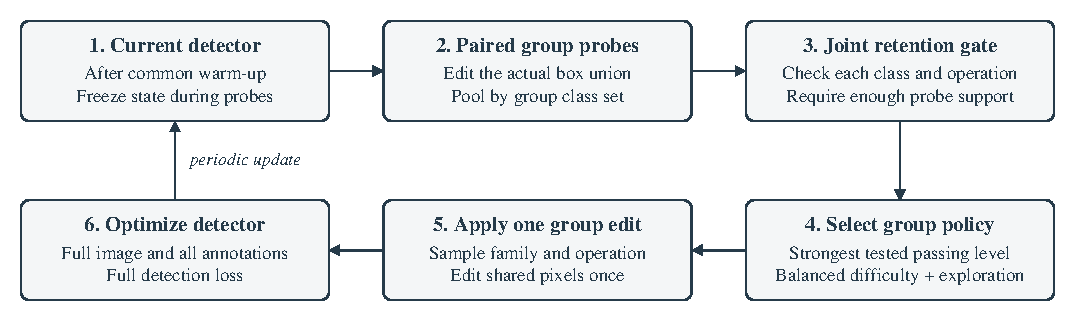
\includegraphics[width=\textwidth]{figures/methodology_framework.pdf}
    \caption{Class-adaptive augmentation framework. Paired probes measure the response to a local union edit and pool feedback by group class set. Class-specific retention determines eligible family strengths, and class-balanced loss feedback determines family-selection probabilities. The selected transformation is applied once to a sampled group before full-image detector optimization.}
    \label{fig:method_framework}
\end{figure*}

\subsection{Overlap Groups and Local Transformations}
\label{sec:method_groups}
% Role: method -- turn shared pixel support into a deterministic augmentation unit.
Overlap groups define the spatial units to which the controller assigns transformations. We first clip boxes to the image boundary and rasterize them using the same pixel-support convention as the edit masks. A graph then connects boxes whose rasterized regions have positive-area intersection. Its connected components form the groups, with an isolated box forming a group of its own. Grouping is based on the annotated box regions, including the pavement context they contain.

% Role: method and advantage -- apply a consistent edit across the complete group union.
For a selected group $G$, the transformation acts on the union $M_G$ of its box regions. Let $T_{o,m}$ denote operation $o$ at discrete strength $m$. The augmented image is
\begin{equation}
    \widetilde{x}=x+\alpha_G\odot\bigl(T_{o,m}(x)-x\bigr),
    \label{eq:local_edit}
\end{equation}
where $\odot$ denotes pixelwise multiplication and $\alpha_G$ is a blending mask with values in $[0,1]$. The mask is zero outside $M_G$ and tapers inward at the union boundary to blend the transformed content with its surroundings. We compute $T_{o,m}(x)$ from the reference image and composite it once over the union. This construction gives shared pixels a single transformation and makes the result independent of box-processing order.

% Role: method -- define the transformation bank and the meaning of strength.
The transformation bank contains two coordinate-preserving families: photometric transformations, comprising brightness, contrast, and gamma adjustment; and blur/noise transformations, comprising Gaussian blur and additive Gaussian noise. Opposite directions, such as brightening and darkening, are represented as separate operations. Each operation has a fixed mapping from ordered levels $m\in\{1,\ldots,M\}$ to its physical parameters, with level zero denoting identity. The same parameter mappings, noise distribution, intensity-clipping rule, and boundary taper are used during probing and training. Because these operations preserve spatial coordinates, the original bounding boxes remain the detection targets.

\subsection{Paired Detection Feedback}
\label{sec:method_feedback}
% Role: method -- isolate candidate effects through paired measurements at one detector state.
Paired probes measure the detector's response to each candidate transformation under a common model state. At each policy update, we select a panel of target-bearing training images, preferring distinct source-image clusters, and sample one group uniformly within each image. Each source-image cluster comprises an image and any linked exact or perceptual duplicate candidates; it is distinct from the within-image overlap group. Panel selection is independent of detection outcomes, and measurements are pooled by the selected groups' class sets. The same panel evaluates the operation--strength grid, with only the target group transformed. Probes run in evaluation mode without gradient updates, keeping detector parameters, normalization statistics, preprocessing, and post-processing fixed. For noise, a fixed set of seeded draws is reused across strength levels.

% Role: method -- define class-specific retention of reference detections.
Detection retention measures the fraction of reference-detected objects that remain detected after transformation. Predictions are matched one-to-one to annotated boxes using the correct class label and fixed confidence and intersection-over-union thresholds. Let $d_j^0$ indicate whether reference object $j$ is detected, and let $d_j^{o,m}$ denote its transformed detection indicator, averaged over draws for a stochastic operation. For class-$c$ objects $\mathcal{P}_{s,c}$ in the target groups of class set $s$, retention is
\begin{equation}
 R_{c\mid s,o,m}=
 \frac{\sum_{j\in\mathcal{P}_{s,c}}d_j^0d_j^{o,m}}
      {\sum_{j\in\mathcal{P}_{s,c}}d_j^0}.
 \label{eq:retention}
\end{equation}
Conditioning on reference detections separates missed detections introduced by the edit from those already present in the reference view.

% Role: method -- specify evidence support and complementary full-image measurements.
The controller uses a class-set policy only when every represented class has the required minimum numbers of reference-detected objects and contributing source-image clusters within that exact class set. Repeated noise draws do not increase either count. Measurements from other class sets cannot supply missing support. An absent or insufficiently supported class set receives identity, and its policy is recomputed from the next panel rather than carried forward from an earlier update. Per-object detection indicators, matched-object IoUs, and full-image false-positive counts are retained alongside the target-group measurements to characterize responses beyond the edited region.

\subsection{Joint Strength Selection}
\label{sec:method_strength}
% Role: method -- regulate family strength using the joint class and operation constraint.
Strength selection uses a joint retention constraint across the classes sharing a group. Let $\mathcal{O}_f$ denote the operations in family $f$, including their directions, and let $\mathcal{A}_{s,f}$ be the set of tested nonzero levels with sufficient probe support for which
\begin{equation}
 \min_{c\in s}\;\min_{o\in\mathcal{O}_f}
 R_{c\mid s,o,m}\geq\rho,
 \label{eq:joint_gate}
\end{equation}
where $\rho$ is the retention threshold. The controller selects the strongest level in this admissible set:
\begin{equation}
 m^*_{s,f}=\max\bigl(\mathcal{A}_{s,f}\cup\{0\}\bigr).
 \label{eq:selected_strength}
\end{equation}
The zero value marks a family as unavailable when no tested level satisfies the constraint. Each level is evaluated independently; selecting the strongest admissible level does not assume that retention decreases monotonically with strength. Both eligibility and strength are recomputed from the current probe measurements at each policy update.

% Role: advantage -- explain why the minimum is taken before family allocation.
The minimum in Eq.~\ref{eq:joint_gate} gives every represented class and operation a separate constraint on the shared strength. For example, a strong blur level is rejected for crack--pothole groups when crack retention falls below $\rho$, even if pothole retention remains high. A weaker blur/noise level is eligible only when both blur and noise satisfy the threshold for both classes. Applying the constraint before family selection prevents an acceptable average from masking a failed class-level check and permits each family to retain its own admissible strength.

\subsection{Class-Balanced Family Selection}
\label{sec:method_allocation}
% Role: method -- measure augmentation difficulty using losses attributable to the target objects.
Family selection uses an auxiliary object-level loss to measure difficulty independently of thresholded detection success. For Faster R-CNN, we assign positive region proposals to annotated objects using the detector's region-of-interest (ROI) matcher and append one ground-truth ROI explicitly assigned to each object. This additional ROI supplies a measurement even when the proposal network misses an object. Each ROI contributes classification cross-entropy plus class-specific Smooth L1 box-regression loss, with equal weights and a Smooth L1 transition parameter of $1/9$; the regression term is summed over the four box coordinates. We average ROI contributions within each object before aggregating objects.

% Role: method and boundary -- separate the auxiliary observer from ordinary predictions and training loss.
Ground-truth ROIs are used only by this auxiliary observer and never enter the predictions used for retention or evaluation. Both views use the same assignment and loss procedure, although their proposal sets may differ. Only losses attributable to target-group objects guide family selection. Background classification and proposal-network losses remain part of ordinary detector optimization. The auxiliary score therefore measures a specific supervised response to the edit, rather than the detector's complete training objective or a guarantee of downstream benefit.

% Role: method -- normalize net class-level changes and aggregate classes equally.
For each class, the difficulty score is the normalized increase in its mean object loss. Let $\bar\ell^0_{c\mid s}$ and $\bar\ell^{o,m}_{c\mid s}$ denote mean losses over the same class-$c$ objects in the reference and transformed views, respectively, with stochastic draws also averaged. We define
\begin{equation}
 A_{c\mid s,o,m}=\operatorname{clip}_{[0,B]}
 \left(\frac{\bar\ell^{o,m}_{c\mid s}-\bar\ell^0_{c\mid s}}
 {\bar\ell^0_{c\mid s}+\delta}\right),
 \label{eq:class_difficulty}
\end{equation}
where $\delta>0$ stabilizes normalization and $B>0$ caps the score. Averaging before clipping retains both positive and negative object-level changes when measuring the net class response. Reference-loss normalization adjusts for differences in class loss scale. The score for family $f$ at its selected strength is
\begin{equation}
 D_{s,f}=\frac{1}{|s|\,|\mathcal{O}_f|}
 \sum_{c\in s}\sum_{o\in\mathcal{O}_f}
 A_{c\mid s,o,m^*_{s,f}}.
 \label{eq:family_score}
\end{equation}
The two averages give equal weight to each represented class and to each operation within the family, so classes with more boxes do not dominate family allocation.

% Role: method -- combine difficulty-weighted sampling with continued exploration.
The sampling distribution combines difficulty weighting with uniform exploration over eligible families. For nonempty $\mathcal{E}_s=\{f:m^*_{s,f}>0\}$,
\begin{equation}
 p(f\mid s)=(1-\varepsilon)
 \frac{\exp(D_{s,f}/\tau)}
      {\sum_{h\in\mathcal{E}_s}\exp(D_{s,h}/\tau)}
 +\frac{\varepsilon}{|\mathcal{E}_s|},
 \label{eq:family_probability}
\end{equation}
where $\tau>0$ controls the concentration of the difficulty-weighted component and $0<\varepsilon\leq1$ sets the uniform exploration weight. The uniform term gives every eligible family a nonzero probability. After selecting a family, we sample one of its operations uniformly and apply it at $m^*_{s,f}$. Stochastic operations use a fresh draw from the same distribution used in probing. If no family is eligible, the group receives the identity transformation.

\subsection{Training Procedure and Evaluation Design}
\label{sec:method_evaluation}
% Role: method -- integrate the selected group edit with full-image detector optimization.
Local augmentation is integrated into training through a fixed application probability $q$. After warm-up, an image selected for augmentation contributes one uniformly sampled group, whose class-set policy determines the family, operation, and strength. Other groups remain unchanged on that visit and can be selected on subsequent visits. This matches the single-group intervention used in probing. The complete image and all its annotations contribute to the detector's classification, localization, and background losses. Images without target boxes receive no local edit and retain background supervision. Policy updates use forward measurements, while detector updates minimize the full detection loss.

% Role: method -- distinguish adaptation data from model-selection and evaluation data.
Policy adaptation uses only training annotations and training-image probes. Validation selects the detector checkpoint and supplies development comparisons; it does not supply the online retention or difficulty measurements. Test data are excluded from optimization, probing, and checkpoint selection. Separate random-number streams govern image order, augmentation decisions, and probe selection. Saving the controller state with the detector, optimizer, and random-number states preserves the adopted policy across interrupted training.

% Role: evidence and boundary -- connect the implemented comparisons to the research question.
The evaluation contrasts identity augmentation, fixed image-level augmentation, fixed local augmentation, online shared local control, and online class-adaptive local control. Section~\ref{sec:experimental_setup} specifies the common detector protocol and the comparisons' scope. Detection retention constrains the measured response of the current model; neither passing this constraint nor increasing the auxiliary loss establishes semantic preservation or improved generalization.

\section{Experimental Setup}
\label{sec:experimental_setup}

\subsection{Dataset and Partitioning}
\label{sec:setup_data}
% Role: setup -- define the data population, exclusions, and target conventions.
We use complete annotated images from the seven RDD2022 source groups: China Drone, China MotorBike, Czech, India, Japan, Norway, and the United States~\cite{arya2024rdd}. The four foreground labels are D00, D10, D20, and D40. Auditing the 38,385 available images excludes one exact duplicate with conflicting annotations and one image with an ambiguous class label; one zero-area target box is removed while retaining its image and remaining targets. The resulting pool contains 38,383 images and 55,002 target objects. Valid difficult and truncated targets are retained as ordinary ground truth. Images without annotations for the four target classes remain in the dataset as background-supervision examples; this designation does not establish that their pavement is damage-free.

% Role: setup and limitation -- explain the frozen split and its independence boundary.
The study uses a custom mixed-source split of 26,863 training, 5,760 validation, and 5,760 reserved test images, containing 38,530, 8,225, and 8,247 target objects, respectively. Exact matches and screened perceptual-similarity links define source-image components that are assigned wholly to one partition. Existing test assignments are preserved, components with prior training exposure remain in training, and unassigned groups are balanced within each source toward a 70/15/15 allocation. Six validation images linked to components with training exposure are reassigned to training through this rule. The manifests and exclusions are fixed before detector training. This grouping reduces leakage through identified related images but does not establish independence of all roads or capture sequences, and the split does not measure unseen-country transfer.

\subsection{Detector and Optimization}
\label{sec:setup_detector}
% Role: setup -- specify the common detector and image representation.
All conditions use Faster R-CNN with a ResNet-50 feature pyramid backbone, initialized from the same COCO-pretrained weights. The ROI predictor is replaced with a five-class head for the four damage categories and background. All backbone stages are trainable, with frozen batch-normalization statistics. Each run starts afresh from this initialization rather than continuing a previous condition's checkpoint. Images are decoded in stored orientation, converted to RGB, resized with aspect ratio preserved, and centered in a $640\times640$ canvas with padding value 114. Bounding boxes follow the actual horizontal and vertical resize factors; predictions are mapped back to original image coordinates for evaluation.

% Role: setup -- fix optimization and distinguish learning-rate warm-up from policy warm-up.
Training uses 20 epochs, a batch size of four, and stochastic gradient descent with momentum 0.9 and weight decay $5\times10^{-4}$. The base learning rate is 0.0025, reached through a linear warm-up over 1,000 optimizer steps from $0.001$ times that value. It decreases by a factor of ten after epochs 12 and 16. The complete budget is 134,320 optimizer steps and 537,260 training-image presentations per condition. Augmented conditions use an unaugmented first epoch before enabling their policies. Computation uses FP32 with automatic mixed precision and TF32 disabled. The implementation uses PyTorch 2.3.0, TorchVision 0.18.0, and one NVIDIA A10 GPU per run on CCAST.

\subsection{Augmentation Conditions}
\label{sec:setup_conditions}
% Role: comparison -- define the five conditions and the controlled spatial contrast.
Table~\ref{tab:augmentation_conditions} defines the five comparison conditions. Identity applies only the common preprocessing. The fixed image-level and fixed local conditions share the same operation parameters and sampling rule: each family has probability $1/2$, followed by a uniform draw among its operations at level two. Their difference is whether the edit covers the resized image content or one sampled overlap-group union. Across all augmented conditions, only target-bearing images are eligible, with application probability $q=0.5$ after the first epoch; images without target boxes remain unchanged. Thus, the spatial comparison does not also introduce augmentation of background-only images.

\begin{table*}[t]
\caption{Augmentation Conditions Under a Common Detector Training Protocol}
\label{tab:augmentation_conditions}
\centering
\small
\setlength{\tabcolsep}{4pt}
\renewcommand{\arraystretch}{1.12}
\begin{tabularx}{\textwidth}{@{}p{0.21\textwidth}p{0.20\textwidth}p{0.23\textwidth}Y@{}}
\toprule
\textbf{Condition} & \textbf{Spatial scope} & \textbf{Feedback pooling} & \textbf{Strength and family selection} \\
\midrule
Identity & No augmentation & None & Identity only \\
Fixed image-level & Full resized content & None & Level two; uniform families \\
Fixed local & One overlap-group union & None & Level two; uniform families \\
Online shared local & One overlap-group union & All probe groups, by class & Shared family strengths and probabilities \\
Online class-adaptive local & One overlap-group union & Exact group class set, by class & Class-set-specific strengths and probabilities \\
\bottomrule
\end{tabularx}
\end{table*}

% Role: comparison and limitation -- identify what the online contrasts can isolate.
The two online conditions use identical probe panels, group choices, candidate transformations, update schedules, and numerical thresholds. The shared controller pools groups across class sets and applies its retention constraint to all four classes. The class-adaptive controller pools only groups with the same exact class set and constrains each class represented in that set. This contrast changes feedback pooling and policy routing, including the support available to each policy. The fixed-local comparison additionally changes access from one prescribed strength to three candidate strengths, so it cannot isolate online adaptation independently of the candidate range. The fixed recipes are specified before their runs and are not selected by a validation policy search.

\subsection{Transformations and Controller Settings}
\label{sec:setup_controller}
% Role: implementation -- define operation parameters and the shared rendering convention.
The operation bank contains six photometric operations and two blur/noise operations, with the three strength levels in Table~\ref{tab:operation_levels}. Brightness scales RGB values; contrast scales deviations from the full-content mean luminance; gamma applies the exponent to values normalized to $[0,1]$. Noise is independently Gaussian for each pixel and channel. Operations act on stored RGB code values, followed by clipping and rounding to 8-bit intensities. For local edits, clipped boxes are rasterized using floor at the minimum edges and ceiling at the maximum edges. The union mask has opacity 0.5 on its outer eight-neighbor boundary and 1 in its one-pixel-eroded interior; one-pixel-wide regions retain opacity 0.5. Padding remains unchanged.

\begin{table}[t]
\caption{Operation Parameters at the Three Candidate Strengths}
\label{tab:operation_levels}
\centering
\small
\setlength{\tabcolsep}{3pt}
\renewcommand{\arraystretch}{1.12}
\begin{tabularx}{\columnwidth}{@{}Yccc@{}}
\toprule
\textbf{Parameter} & \textbf{Level 1} & \textbf{Level 2} & \textbf{Level 3} \\
\midrule
Brightness down/up & 0.9/1.1 & 0.8/1.2 & 0.7/1.3 \\
Contrast down/up & 0.9/1.1 & 0.8/1.2 & 0.7/1.3 \\
Gamma brighten/darken & 0.9/1.1 & 0.8/1.2 & 0.7/1.3 \\
Gaussian blur radius (px) & 0.4 & 0.8 & 1.2 \\
Gaussian noise std.\ (RGB/255) & 0.01 & 0.02 & 0.03 \\
\bottomrule
\end{tabularx}
\end{table}

% Role: implementation -- specify the probe budget, support, and fixed numerical choices.
Controller updates occur before epochs 2, 4, \ldots, 20, with the selected policies held fixed between updates. Each update uses 256 target-bearing training images in total, not 256 per class set. Images are ranked using keyed pseudorandom draws, prioritizing distinct source-image clusters before filling from unused images, and one group is selected uniformly in each image. Gaussian noise uses two independent draws, each reused across strength levels; the other operations use one view per level. Table~\ref{tab:controller_settings} gives the remaining settings. They are fixed engineering choices for this comparison, rather than validation-optimized estimates. The minimum support prevents decisions based on only one or two detections, but does not supply a statistical precision guarantee. Unsupported or inadmissible class sets receive identity without borrowing a shared policy or resampling another group.

\begin{table}[t]
\caption{Settings Shared by the Two Online Controllers}
\label{tab:controller_settings}
\centering
\small
\setlength{\tabcolsep}{4pt}
\renewcommand{\arraystretch}{1.12}
\begin{tabularx}{\columnwidth}{@{}Yl@{}}
\toprule
\textbf{Setting} & \textbf{Value} \\
\midrule
Unaugmented warm-up & 1 epoch \\
Policy updates before epochs & $2,4,\ldots,20$ \\
Probe panel size per update (total) & 256 images \\
Noise draws per level & 2 \\
Reference detection confidence / IoU & 0.25 / 0.50 \\
Retention threshold $\rho$ & 0.80 \\
Reference support per constrained class & 8 objects, 4 clusters \\
Candidate nonzero strengths $M$ & 3 \\
Loss stabilizer $\delta$ / cap $B$ & 0.1 / 5 \\
Softmax temperature $\tau$ & 0.25 \\
Uniform exploration weight $\varepsilon$ & 0.20 \\
Application probability $q$ & 0.50 \\
\bottomrule
\end{tabularx}
\end{table}

\subsection{Evaluation and Computational Accounting}
\label{sec:setup_evaluation}
% Role: evaluation -- define model selection, metrics, and the held-out boundary.
Evaluation uses unaugmented images and averages precision over the four foreground classes and IoU thresholds $0.50{:}0.05{:}0.95$ (AP50:95). Validation is performed after every epoch, and the checkpoint with the highest validation AP50:95 is selected, retaining the earlier epoch on a tie. The metric implementation is pycocotools 2.0.10; complementary outputs include AP50, AP75, per-class AP, and recall with at most 100 detections. Inference uses a score threshold of 0.001 and class-wise nonmaximum suppression at IoU 0.5. Predicted boxes on images without target annotations are counted separately at confidence 0.25. Validation scores are development estimates subject to checkpoint selection; the reserved test partition is excluded from this comparison.

% Role: limitation -- bound conclusions by replication and the development design.
The comparison uses one initialization and sampling seed, 42, with common data order, optimizer settings, and checkpoint-selection rules. Keyed augmentation and probe draws are separated from the detector's random-number stream, but CUDA execution is not constrained to produce identical trajectories. Consequently, small differences cannot be separated from training variability by this design, and the comparison does not estimate between-seed uncertainty. It also does not independently ablate the retention gate, family-specific strength, or difficulty-based allocation.

% Role: cost -- distinguish equal optimizer budgets from the added cost of online feedback.
The optimizer budget is identical across conditions, while online control adds forward computation. Each probe image requires one reference view and 27 transformed views: seven deterministic operations at three levels and two noise draws at each of three levels. Ten updates over 256 images therefore require 71,680 additional image forwards per online condition, plus the auxiliary ROI-head evaluations. Total run time and probe time are recorded separately, alongside policy support, retention, chosen strengths, family probabilities, and actual edit exposure. Equal augmentation opportunities do not imply equal numbers of modified images, because an online policy can select identity.

\bibliographystyle{IEEEtran}
\bibliography{references}

\end{document}
